% Chapter 3

\chapter{Description of the proposed solution} % Main chapter title

\label{Chapter3} % For referencing the chapter elsewhere, use \ref{Chapter1} 

\lhead{Chapter 3. \emph{Description of the proposed solution}} % This is for the header on each page - perhaps a shortened title

%----------------------------------------------------------------------------------------

This chapter describes the proposed solution. The developed system needs to be able to complete each of the steps stated in the Problem Definition. The system general functioning scheme includes the proposed solutions for all the steps, and is depicted in Figure \ref{fig:scheme}  It will be explained in detail trough the sections in this Chapter. 

The classification of the data in this Chapter is based on the definitions of \emph{new}, \emph{strange} and \emph{interesting}. proposed in page \pageref{definitions}, and that were further developed in \pageref{new}.

\begin{figure}[h]
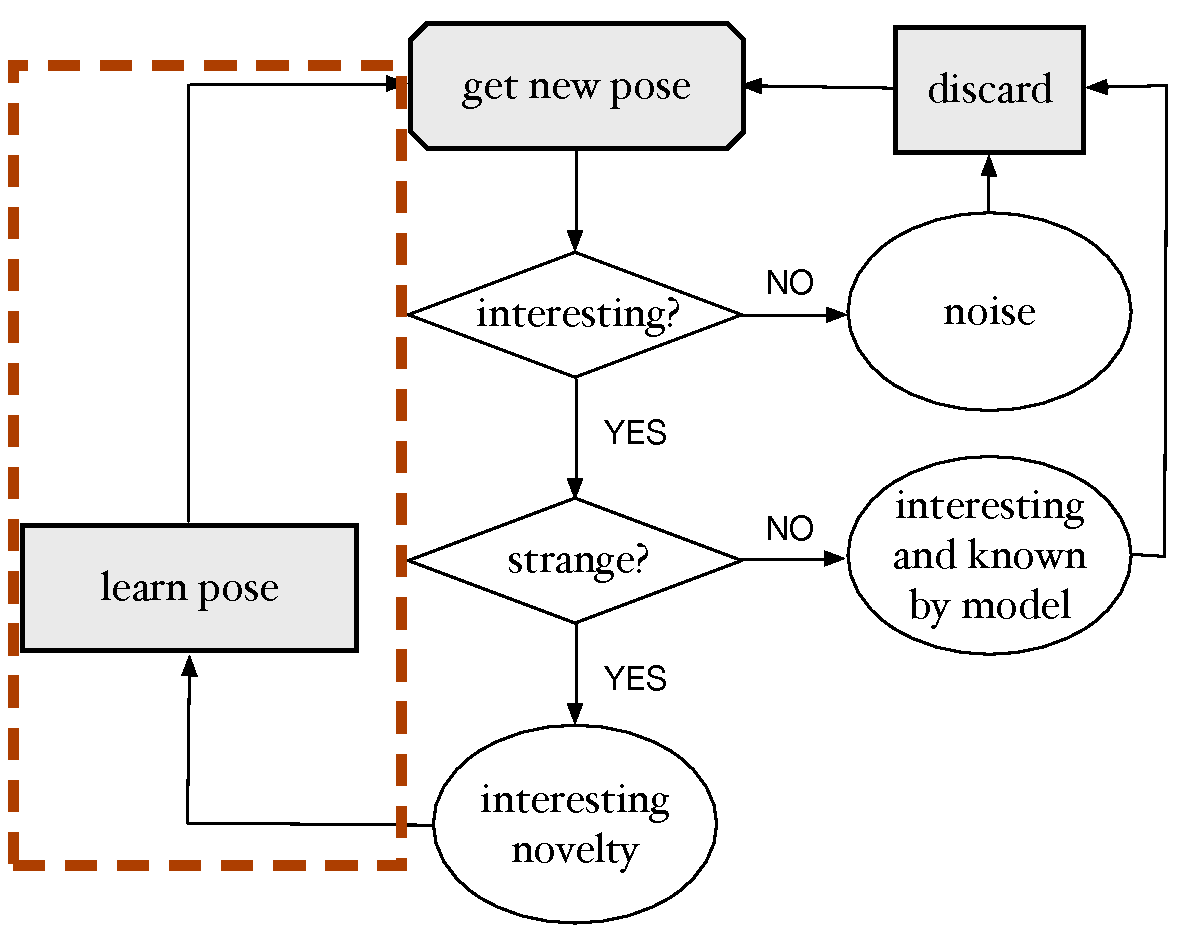
\includegraphics[width=10cm]{Figures/Esquema}
\centering
\caption[System general scheme functioning.]{System general scheme functioning. The new entry is first tested to be classified as interesting or noise. If it is interesting, it is then tested to check if it is strange, resulting in an interesting novelty, or if it is known. Noisy and know entries are discarded, while novelties are learned \label{fig:scheme}.}
\end{figure}

The process begins with the arrival of a new pose data from the modules of the Kinect. That entry is tested against all other data entries received up to that point. If the result is positive, then the entry is considered interesting, as defined in page 5. After that, the entry is be tested against the knowledge base to determine if it is strange, again as defined in page 5. If the result is positive in this second test, the entry is classified as novelty, raising the alerts to the programmer and to other learning modules. The entry is then learned by the system by adding it to the knowledge base.   

If the new pose data is regarded as not interesting it is classified as noise, and it is just kept in the dataset of all entries received. If it is regarded as not strange, it is classified as known and is also kept in the dataset of all entries received. After the new data is classified and added to the correspondent dataset, the system waits for the arrival of another new pose data.     

Not to waste computational resources, the system checks first if the new data is interesting instead of strange. The reason behind this is that it would not make sense to use time and computational power in checking if a data entry is strange, if it is later detected as not interesting. With this structure, the system filters first the data so we can get rid of noisy entries in the first step, and it does not make extra computations unnecessarily. 

The steps presented in the previous section can be identified in Figure \ref{fig:scheme} as well. Quantifying the interest of the stimuli is represented as the decision 'interesting?' and quantifying the strangeness is identified in the decision 'strange?'. Learning from novel stimuli is depicted as the process 'learn pose' after the pose is detected as novel. Working autonomously is related with the functioning system working in a continuous loop; and being interactive involves that the results of \emph{noise}, \emph{known} and \emph{novelty} should be transmitted to the user. Note that the curiosity level is the threshold that determines the answers for the decisions 'interesting?' and 'strange?', as there are two tests and the paramenters considered for each one are different, the system needs two curiosity levels.

The designed solution for each of the steps independently will now be explained in detail in the following sections. Altought the general scheme involves first the noise filtering step and then the strangeness evaluation, the sections present first the strangness evalutation and then the noise filtering. This is because the strangeness evaluation method is more intuitive, and helps to understand concepts that will be later used in the noise filtering method.

\section{Enabling the system to evaluate the strangeness of a stimuli} \label{3.1}

The step of quantifying the strangeness of a stimuli allows the system to identify the new data entry as known or novelty. In Figure \ref{fig:sche_strange} the process is located in the general scheme of the system. 

\begin{figure}[h]
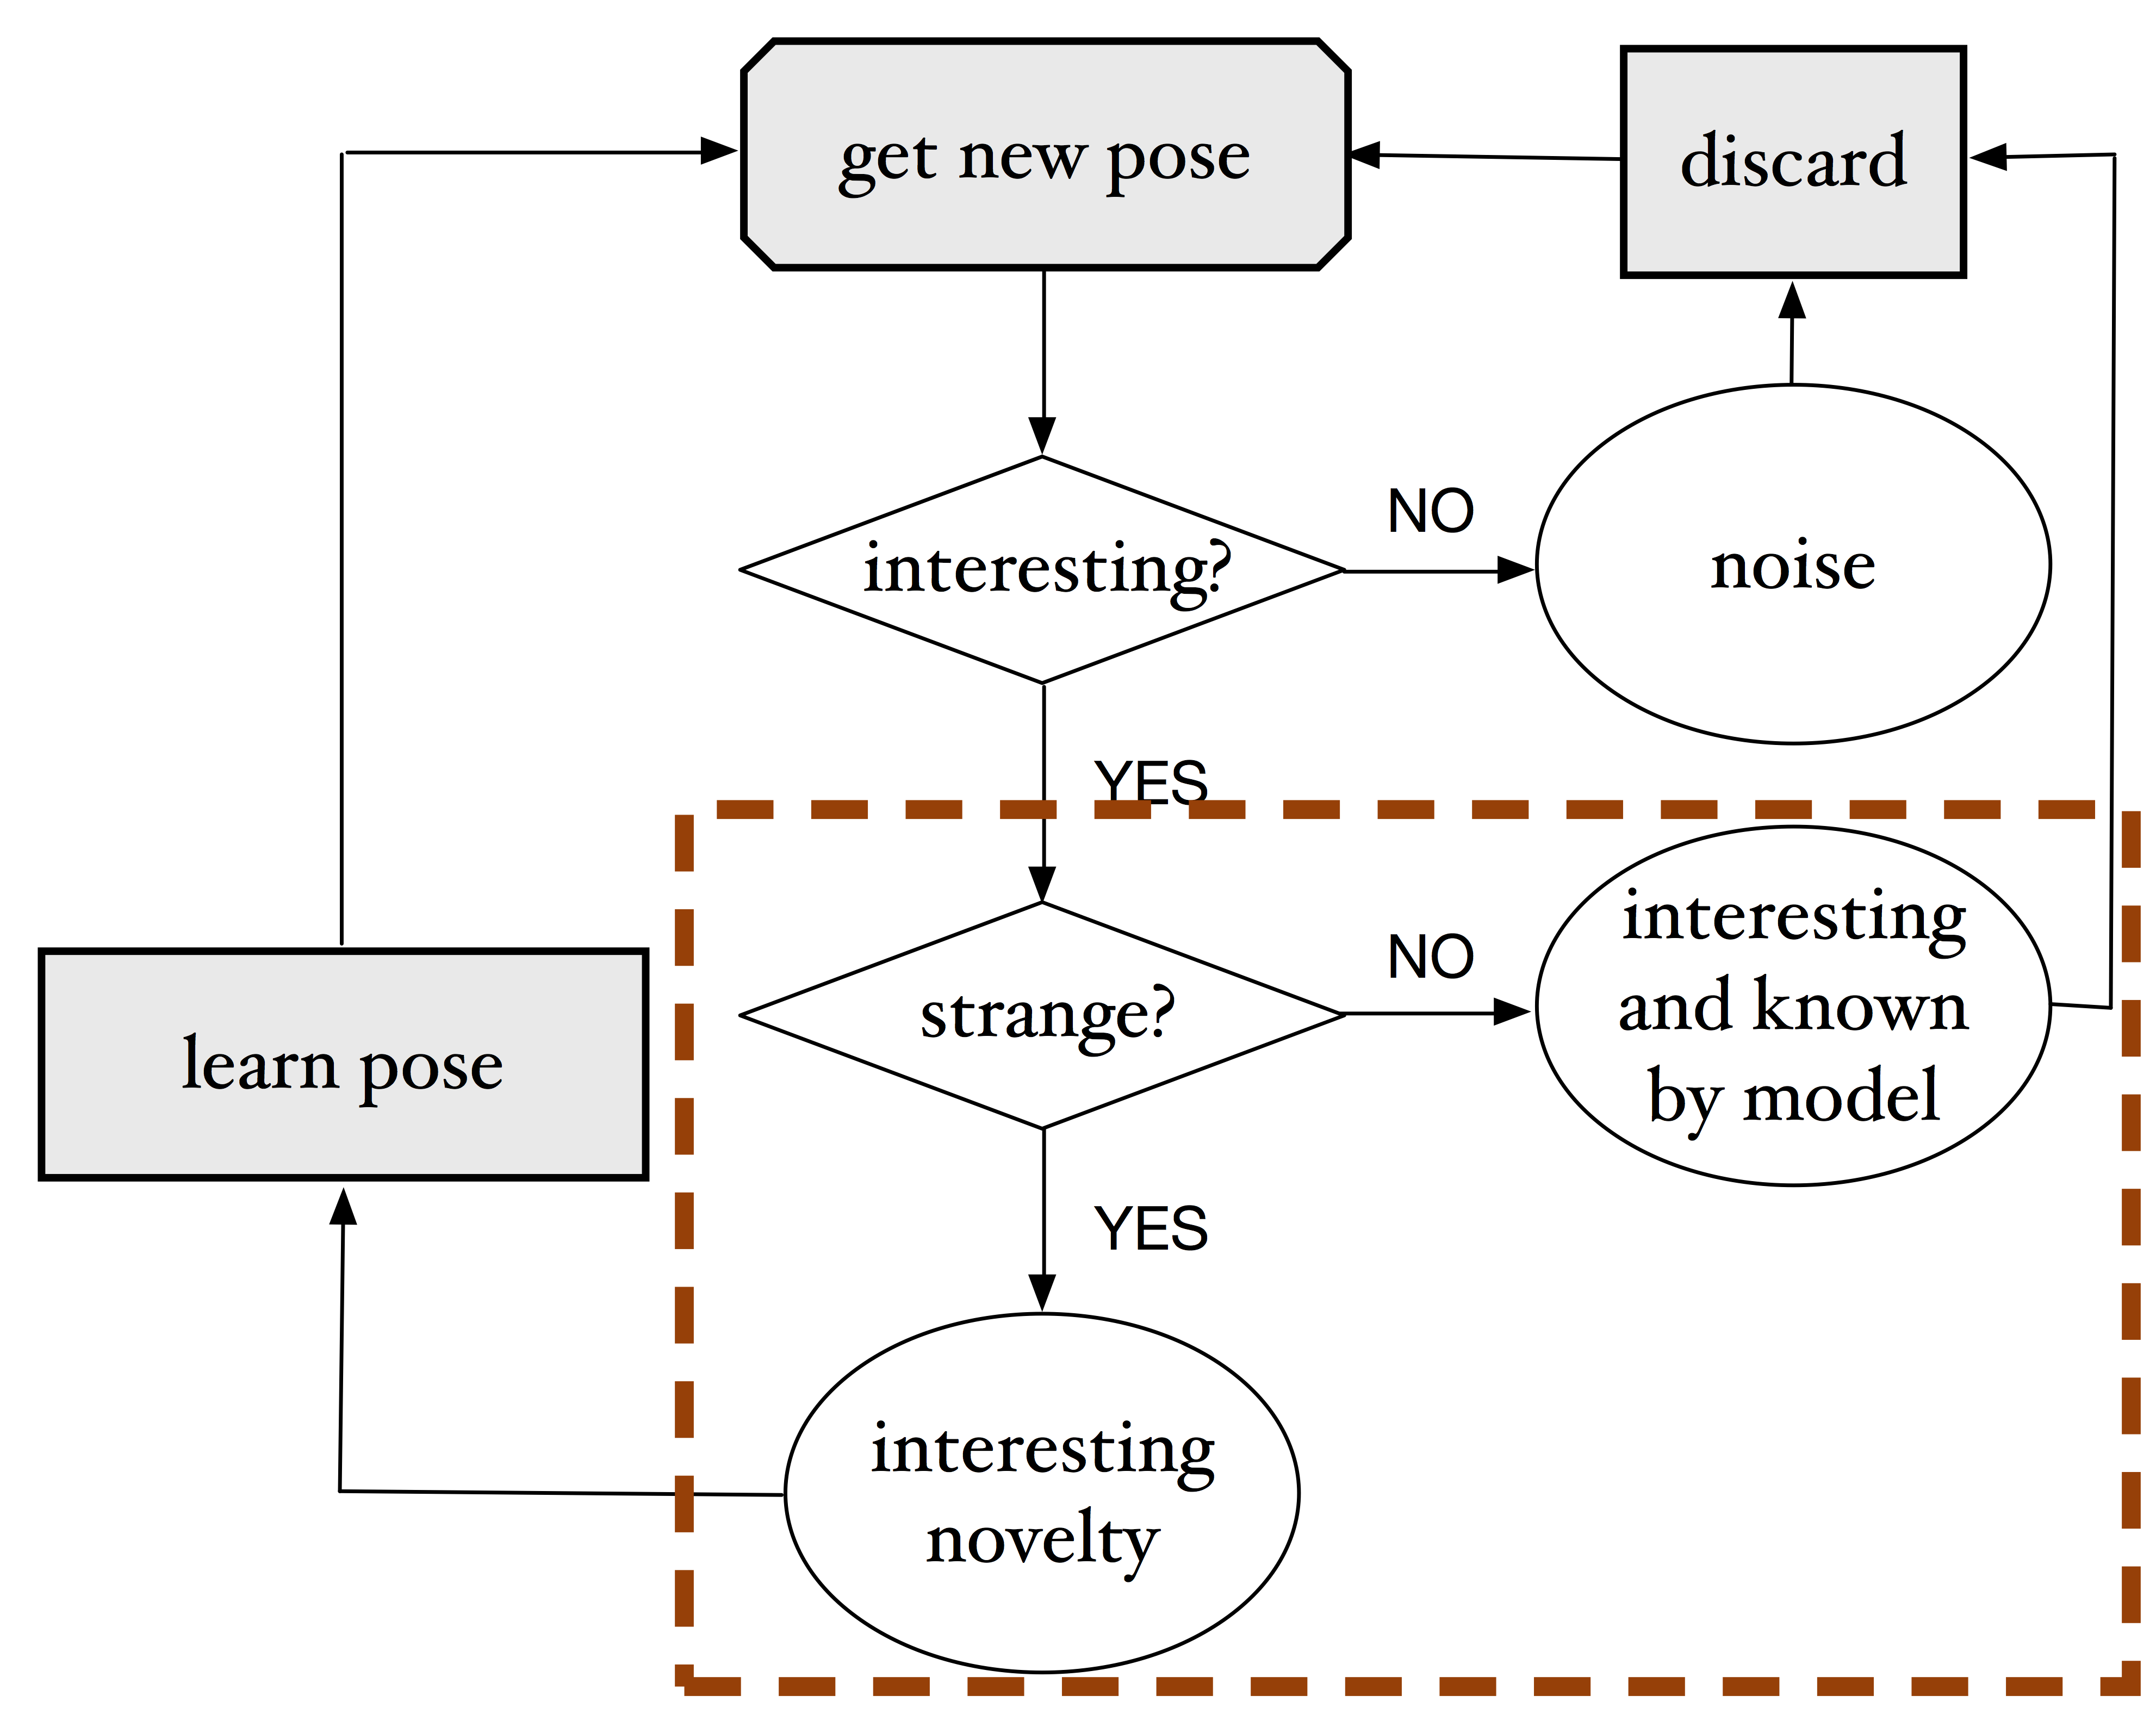
\includegraphics[width=9cm]{Figures/Esquema_strange}
\centering
\caption{Strangeness evaluation step located in the general scheme. \label{fig:sche_strange}}
\end{figure}

This process, as mentioned in Section \ref{2.1}, consists on obtaining the model of normality M(\( \theta  \)), where \( \theta  \)
representing the free parameters of the model. Then this model is used to assign a novelty score, $z(x)$, to new data $x$. 

Some novelty detection methods predict directly a label, \emph{normal} or \emph{abnormal}, when a new entry is detected. Some others provide an score of how well a entry fits into the model. In this later cases, from the model of normality, we can obtain a novelty threshold. This will be further explained in the following sub-sections.

The following rule applies, where $z$ is the novelty score of a new instance $x$ and $k$ is the novelty threshold.:
\medskip

\begin{equation}
	z(x) \geq  k 
\end{equation}

If this condition holds, then $x$ is considered as \emph{abnormal}. This equation was retreived from \cite{Pimentel2014}. 

\subsection{Model of normality}

The normal dataset consists of the poses that have been considered normal and were learned at some point. The model of normality is generated by the novelty detection algorithms, using the normal set as the training set. The algorithms used in this Thesis are explained in Section \ref{3.6}. The normal set is expanded as the system learns new poses. The system learns whatever the user teaches it. We consider that the learned poses are a consistent base of knowledge. 

\subsection{Obtaining the novelty score}

The model is obtained using one-class classification methods. These classifications methods allow to compute an score of how well each instance fits the calculated model. The score is calculated differently for the distinct methods used in this Thesis, how these methods operate will be further explained in Section \ref{3.6}.

If we consider the normal dataset N1, and fit a model $M$ with these entries:
\medskip

\centerline{$ N_1 = [n_1, n_2, n_3,...,n_m]  $ and $ M(N_1)$ }

We can obtain a fitting score, from the algorithm, for each of the instances from the model $ M(N1) $ :
\medskip

\centerline{$ scores = [z(n_1), z(n_2), z(n_3),...,z(n_m)] $}

This set of scores represents a distribution of the scores of the normal entries. This distribution can be normalized, as shown in Figure \ref{fig:normal_d}, obtaining a mean $\mu$ and a standard deviation $\sigma$. 

\begin{figure}[h]
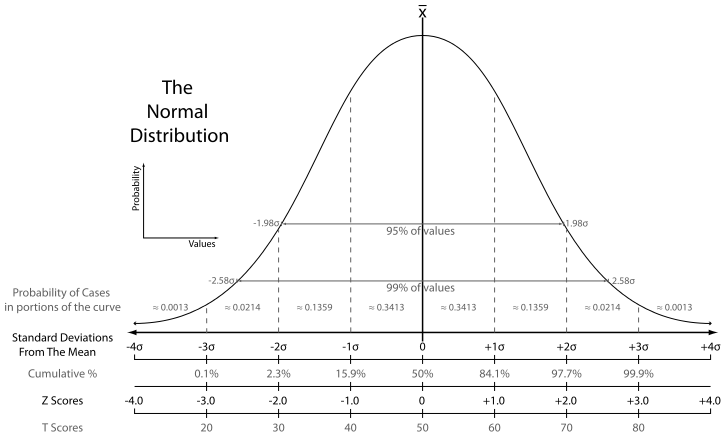
\includegraphics[width=15cm]{Figures/Normal_d}
\centering
\caption[Normal distribution]{Normal distribution, including Standard Deviation and Z score parameters. Retrieved from Wikipedia \cite{standard}. \label{fig:normal_d}}
\end{figure}

A standard score\footnote{The standard score formula can also be denominated the normal score or z score in the literature} of a new entry, $o_1$ \footnote{The convention is using the letter $o$ to label outliers}, can be calculated as follows:

\begin{equation}
standard.score(o_1) = \dfrac{z(o_1) - \mu}{ \sigma}
\end{equation}

Since the distribution is symmetrical, we are interested in the absolute value of this standard score. This is our final $novelty$ $score$.

\begin{equation}
novelty.score(o_1) = abs( \dfrac{z(o_1) - \mu}{ \sigma})
\end{equation}

\subsection{Obtaining the strangeness threshold} \label{3.1.3}

\label{thres1}

The $strangeness$ $threshold$ is obtained from the scores of the normal dataset. We are using the Extreme Value Theorem (EVT) to obtain its value. EVT is a "branch of statistics which deals with extreme deviations of a probability distribution" \cite{Pimentel2014}. It considers extremely large or small values in the tails of the distribution that is assumed to generate the data to obtain the threshold. \cite{Pimentel2014}. This approach can be applied to both \textbf{distance based novelty detection} \textbf{probabilistic novelty detection}, as mentioned in Section \ref{thresholds}.

For example, consider that the novelty threshold is located at one sigma units distance from the mean of the scores in the normal set. Thus, in Figure \ref{fig:normal_sig} can be observed that the strangeness threshold in standard score, also known as z score, for a value of 1 $\sigma$, would be  -1 and 1, where the limits are drawn. Any entry with an score outside the red are will be considered outside the threshold, and thus, abnormal. 

\begin{figure}[h]
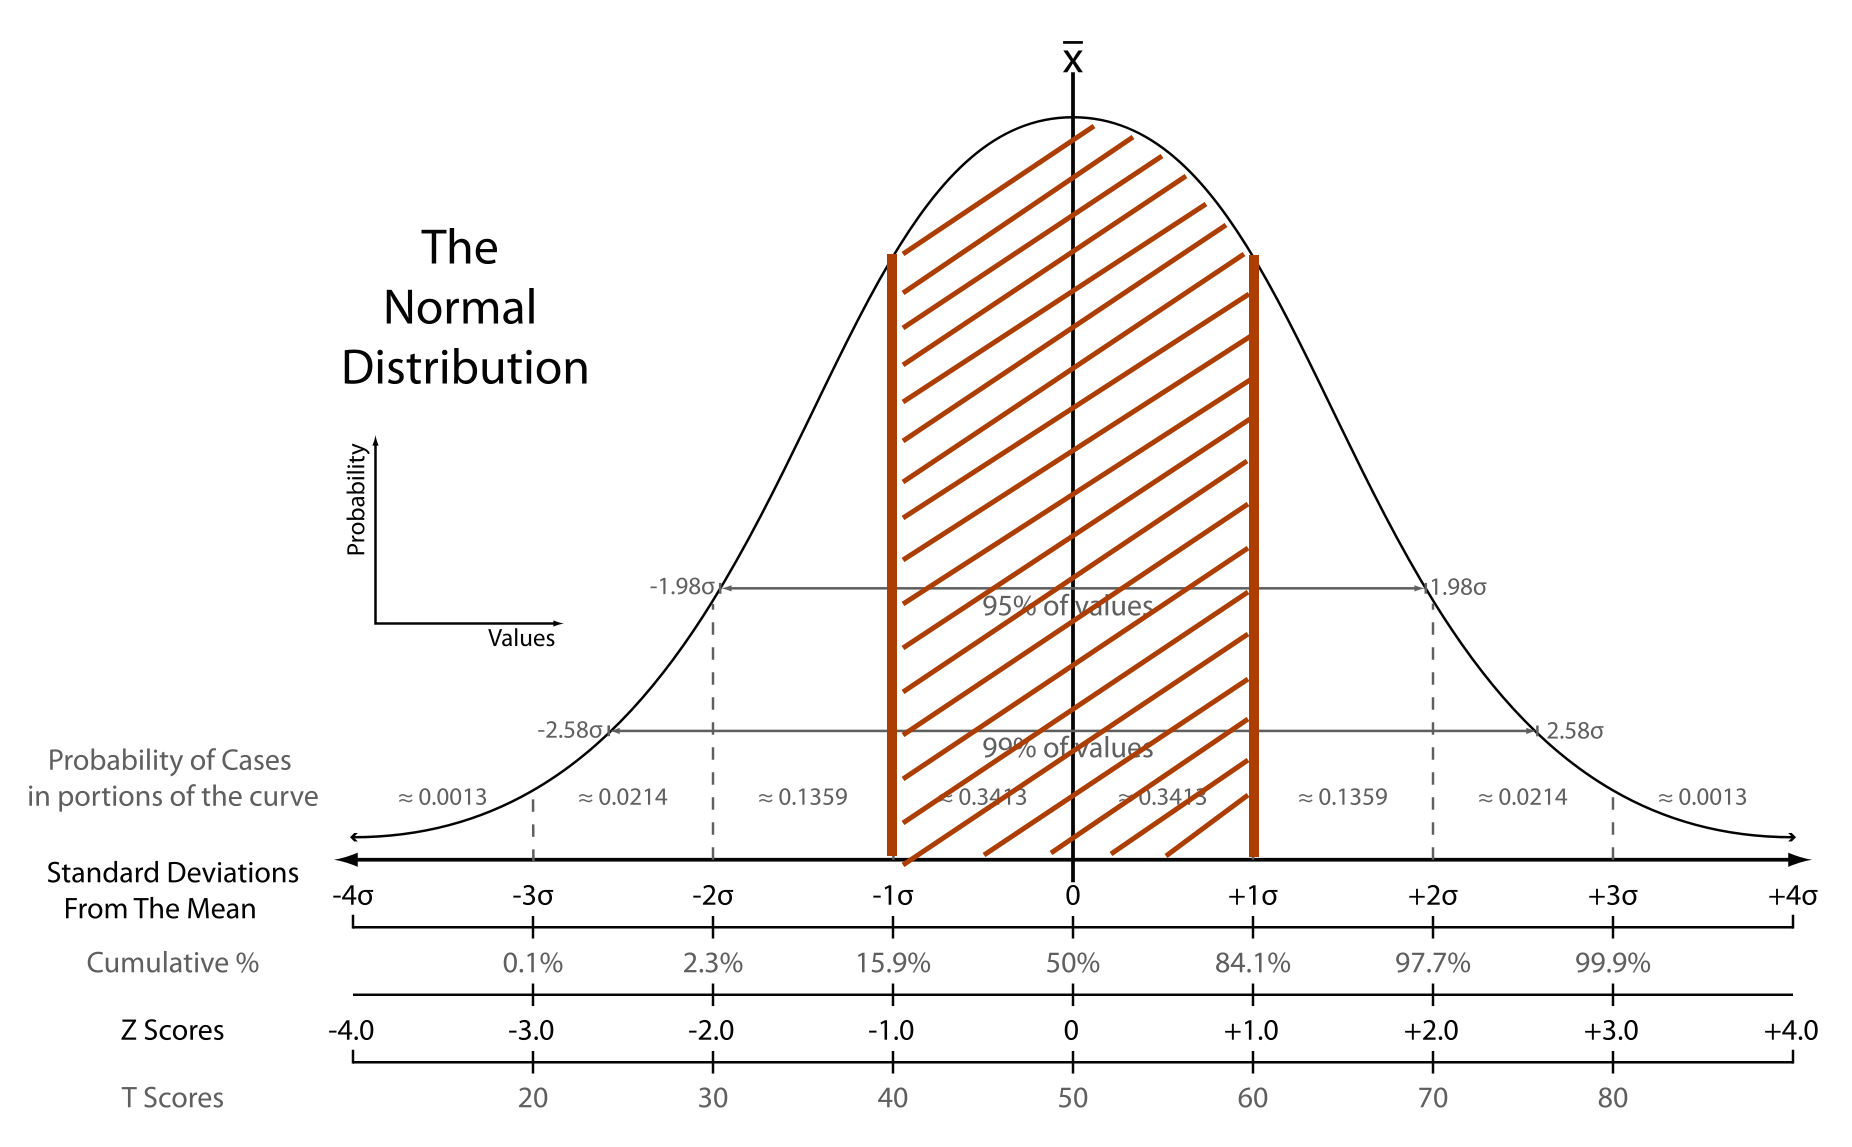
\includegraphics[width=15cm]{Figures/Normal_d_sigma}
\centering
\caption[Normal distribution for one sigma]{Normal distribution for one sigma. The area in red corresponds to the scores in the distribution that are less than 1 sigma units away from the average. Modified and retrieved from Wikipedia \cite{standard}. \label{fig:normal_sig}}
\end{figure}

The equation that represents entries outside the red region is:

\begin{equation}
1 \geq abs( \dfrac{z(o_1) - \mu}{ \sigma} )
\end{equation}

Expading the equation:

\begin{equation}
\begin{split}
z(o_1) \geq \mu +\sigma \\
z(o_1) \leq \mu -\sigma
\end{split}
\end{equation}

In this example, the score of the new data entry is one time $\sigma$ units away from the average value, $\mu$ of the normal scores. A value of one $\sigma$ means that, a new entry is labeled as \emph{normal} if lays within the 68\% of the closests scores to the mean of the dataset. If the standard score is higher than 1, the score $z(o_1)$ can be considered high with respect to 68\% of the normal entries, and it can be classified as strange. 

Imagine we now use a threshold $+K$ and $-K$, instead of +1 and -1. 

\begin{equation}
novelty.score(o_1) = abs( \dfrac{z(o_1) - \mu}{ \sigma})
\end{equation}

\begin{equation}
K \geq abs( \dfrac{z(o_1) - \mu}{ \sigma} )
\end{equation}

If we develop this expression:

\begin{equation}
1 \geq abs( \dfrac{z(o_1) - \mu}{ K \times \sigma} )
\end{equation}

\begin{equation}
\begin{split}
z(o_1) \geq \mu + K \times \sigma \\
z(o_1) \leq \mu - K \times \sigma
\end{split}
\end{equation}

Thus, the standard score for the different entries is inversely proportional to the units of standard deviation, $\sigma$, we consider for the \emph{normal} entries. By increasing the units of sigma considered, we could lower all standard scores, an thus, we would consider as \emph{normal} those scores that were before close to the threshold. 

In consequence, the normalized score can be modified by multiplying the value of $\sigma$ times a K factor, increasing the units of sigma considered. While we can maintain a novelty threshold of +1 and -1.


\section{Enabling the system to filter noise by evaluating the interest of a stimuli} \label{3.2}

The step of quantification of the interest of a stimuli will allows the system to identify the new data entry as noise or interesting. And thus, it is key in the process of detecting and discarding unwanted noise. In Figure \ref{fig:sche_interest} the process is located in the general scheme of the system. 

\begin{figure}[h]
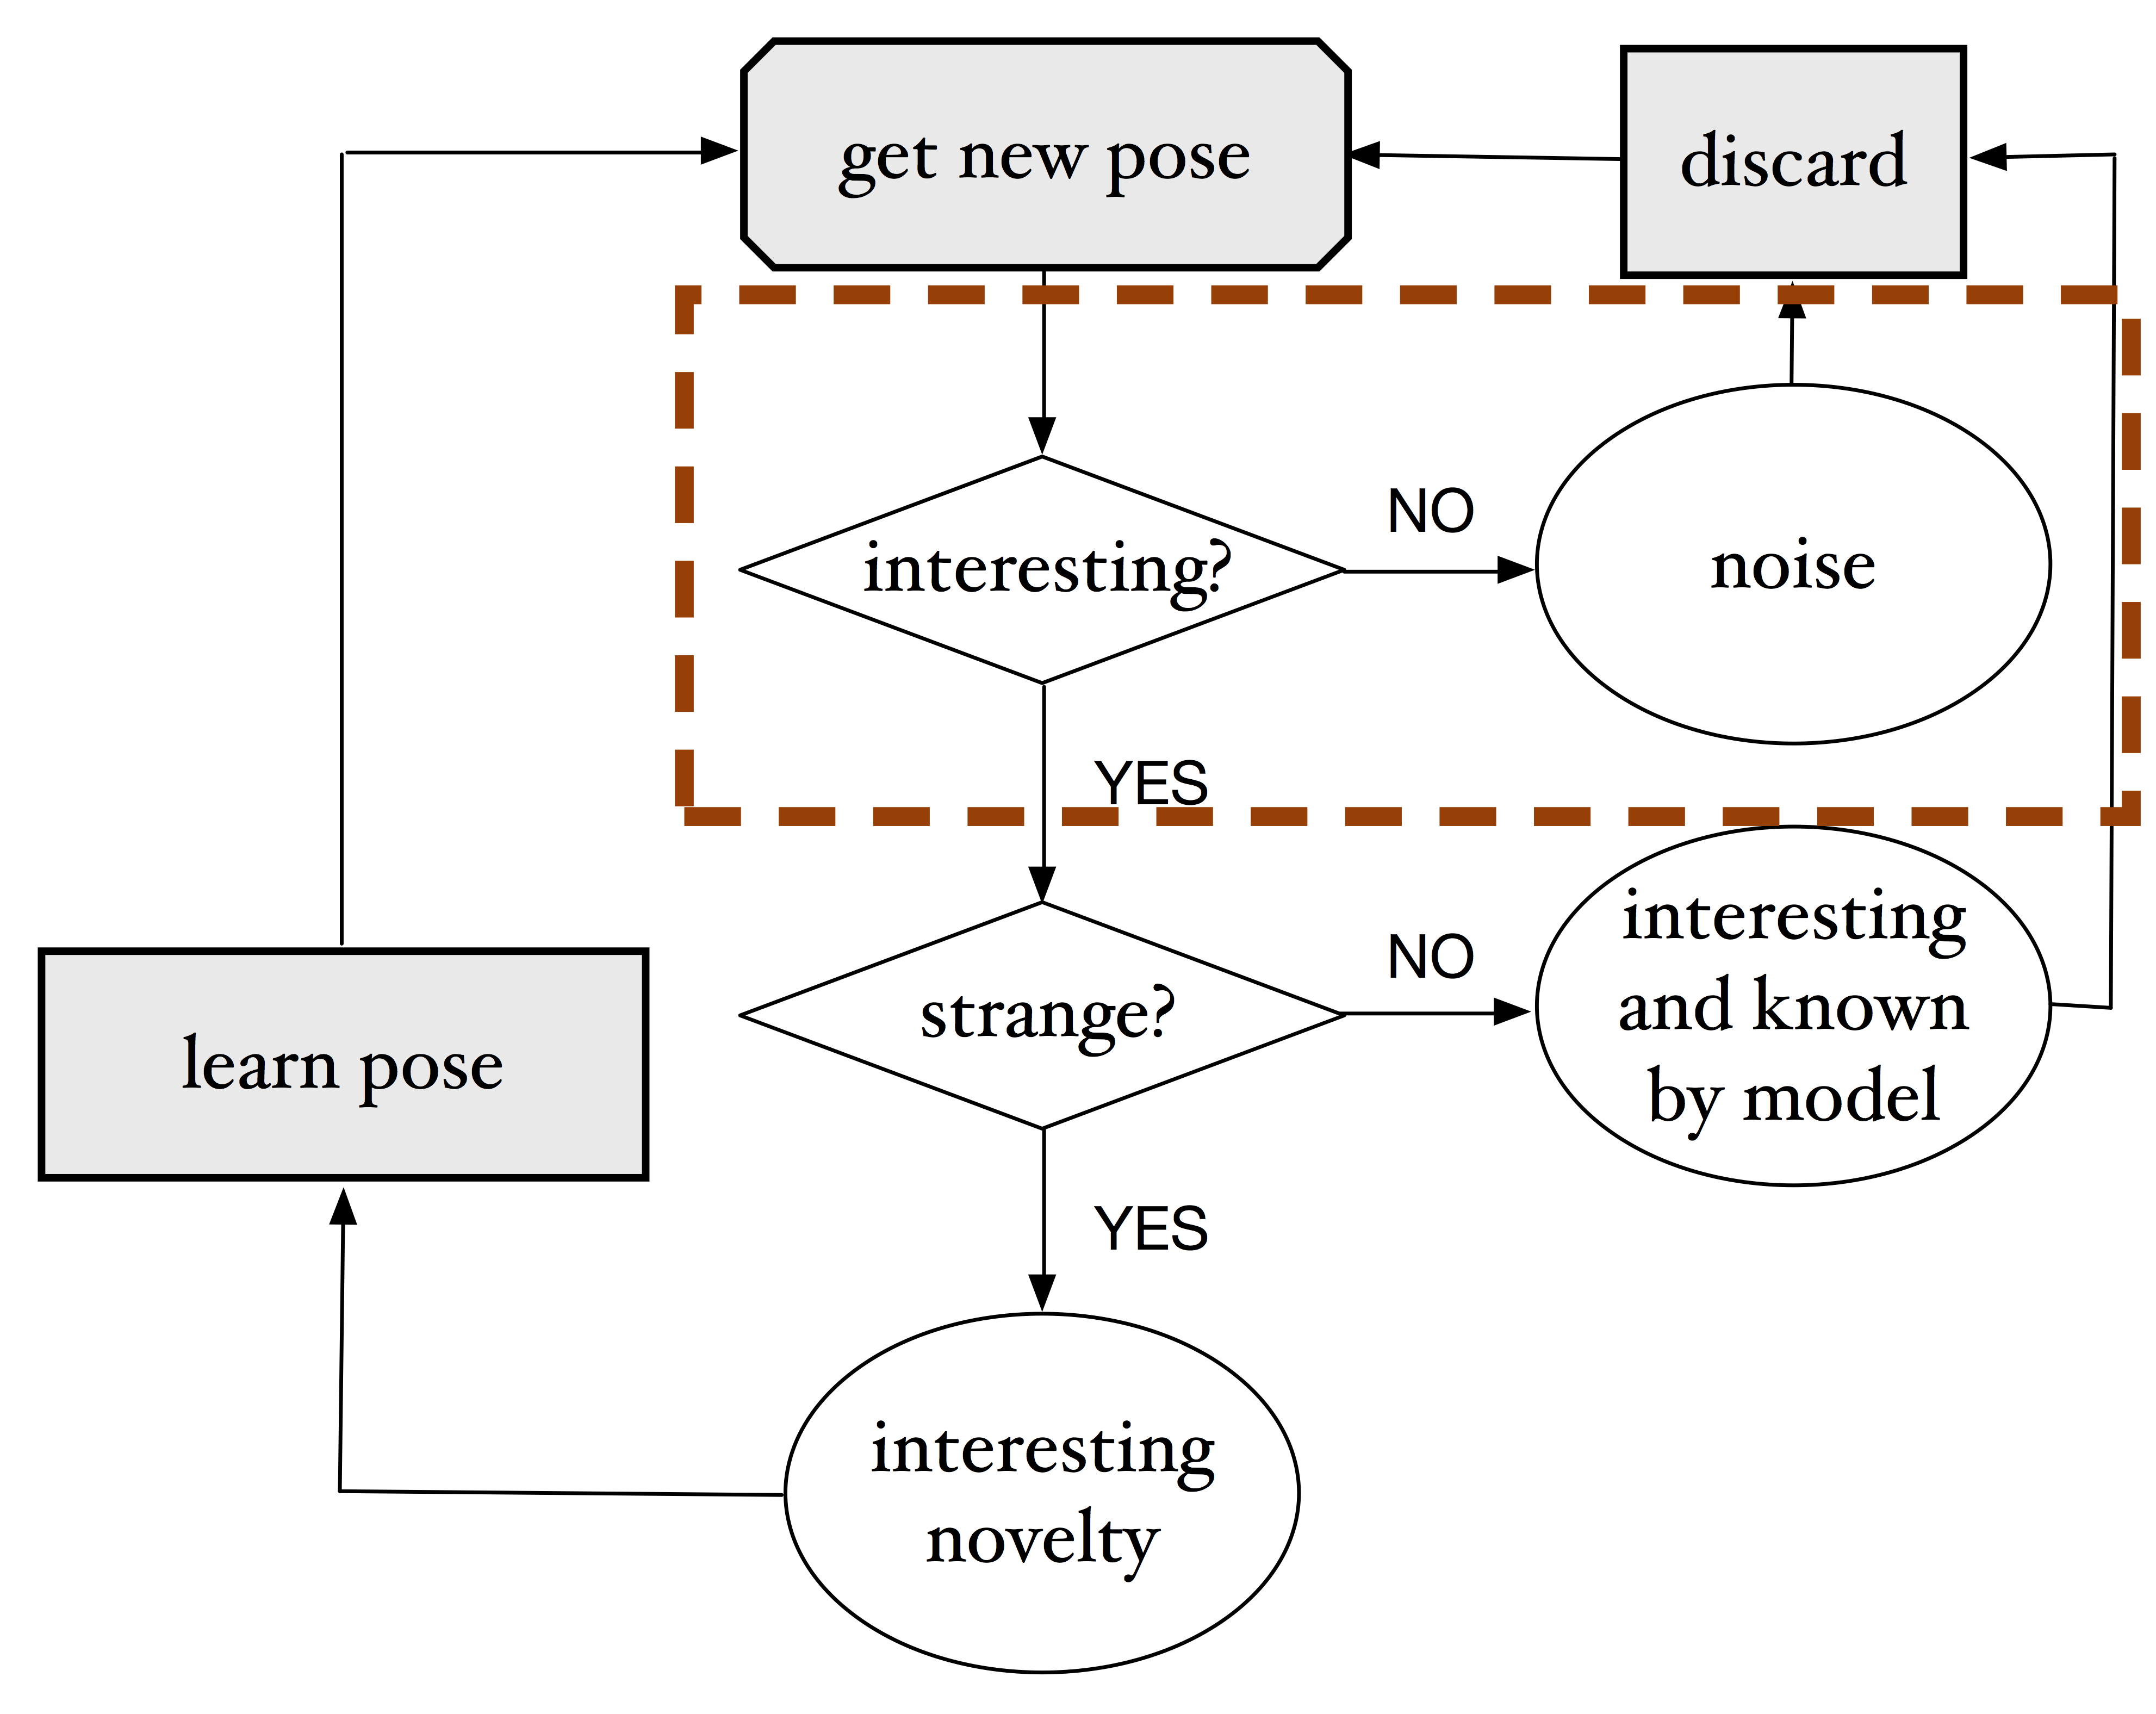
\includegraphics[width=9cm]{Figures/Esquema_interest}
\centering
\caption{Interest evaluation step located in the general scheme. \label{fig:sche_interest}}
\end{figure}

The interestingness of a new data entry depends on what the system has seen before, if it has seen 1000 very similar entries, and 1 new entry is slightly different, probably it will be considered noise. But it also depends on the application, maybe the system needs to be very sensitive to this 1 different entry, and we do not want to discard it. Thus, the system needs to account for all the entries it has ever seen, to see patterns of repetition, and needs to customize its sensitivity. It is important to remember that we are interested in finding out when to ask the user when the system finds something novel, and the application may need that the system does not bother the user too much, so the sensitivity should be low, or on the other hand, we want the system to ask the user a lot, so the sensitivity should be high.

This step can be approached from different perspectives. It can be considered as an outlier detection problem, only that we are interested in detecting when a data entry stops being an outlier and starts being interesting. It can also be considered a clustering problem, in which the objective would be finding out when the data starts forming a cluster around a point, because that would mean that the frequency of appearance around a point is high, and therefore, indicating that this point it is not mere noise but, instead, an interesting data point. 

We can consider all the data ever presented to the system as \emph{normal} in a one-class classification, with a base of knowledge of all the seen entries. Then we can apply a novelty detection method and find a novelty score for new data using the Extreme Value Theorem (EVT). When the data is labeled as \emph{normal}, then it is similar to something that has happened before, it happens frequently enough to be considered interesting. Depending of the novelty detection algorithm used, we will be using the different approaches mentioned in the previous paragraph. 

Figure \ref{fig:plot_out} show this process for One-class classification in a 2D reduction:

In the \textbf{subfigure (a)} we observe the initial dataset, with only one event happening frequently around an area. This event is what we consider the normal knowledge base.

In the second \textbf{subfigure} \textbf{(b)}, we have added new events that happens frequently around an area, and they have formed a new cluster. We now see two clusters of white points, the new cluster of points can be see in the center left side of the image. The model has been recalculated, taking into account all the instances, that are the normal and the new clusters and the outliers. This is the process we follow to evaluate interestingness. We can see how the one class classification applied to all data changes from (a) to (b). In (b), the new cluster is inside the threshold line of the one class classification. This means that the event happens frequently enough to be considered in the one class classification model, modifying it, and thus is interesting. As it is interesting, the system now evaluates the strangeness of the cluster, as explained in the general scheme, Figure \ref{fig:scheme}. 

In the third \textbf{subfigure (c)}, we evaluate the strangenness of the cluster. We build the one class classification model with only the white, normal instances from (a), as explained in Section \ref{3.1}. It can be observed that the new cluster event, in black, is now outside the threshold, and thus, it is considered strange. As the cluster is classified as  \emph{interesting and strange}, the system concludes that it is, indeed, a \emph{novelty}. Detecting a novelty is what sets off the alert to the learning system and to other interaction modules to ask the user about it. The new events are not noise and are cannot be detected as known by the system, so it wants to learn about them to increase the knowledge base and be able to recognize them in the future. 

\begin{figure}[!htb]
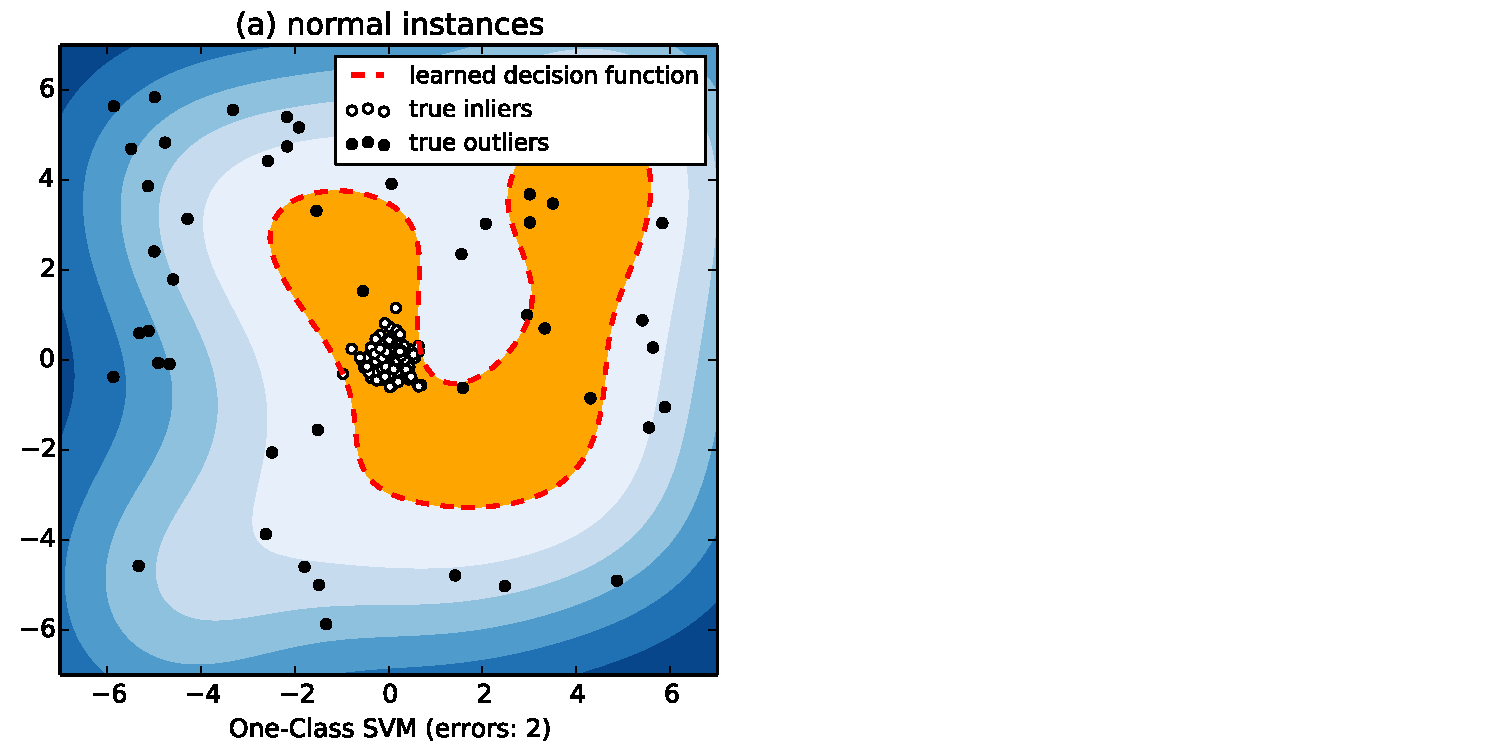
\includegraphics[width=6cm]{Figures/one_class/a}
\centering
\\[\baselineskip]
\minipage{0.5\textwidth}
  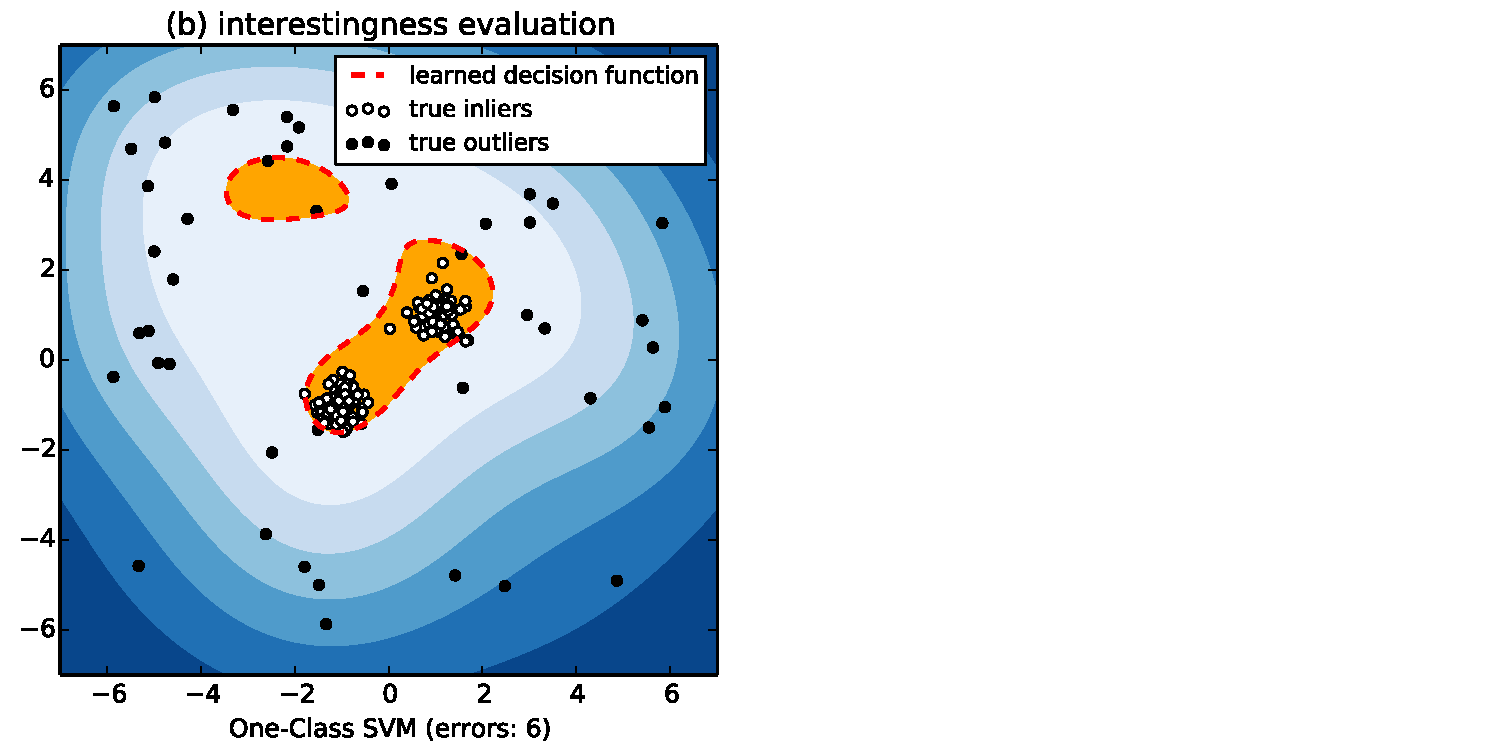
\includegraphics[width=6cm]{Figures/one_class/b}
  \centering
\endminipage\hfill
\minipage{0.5\textwidth}%
  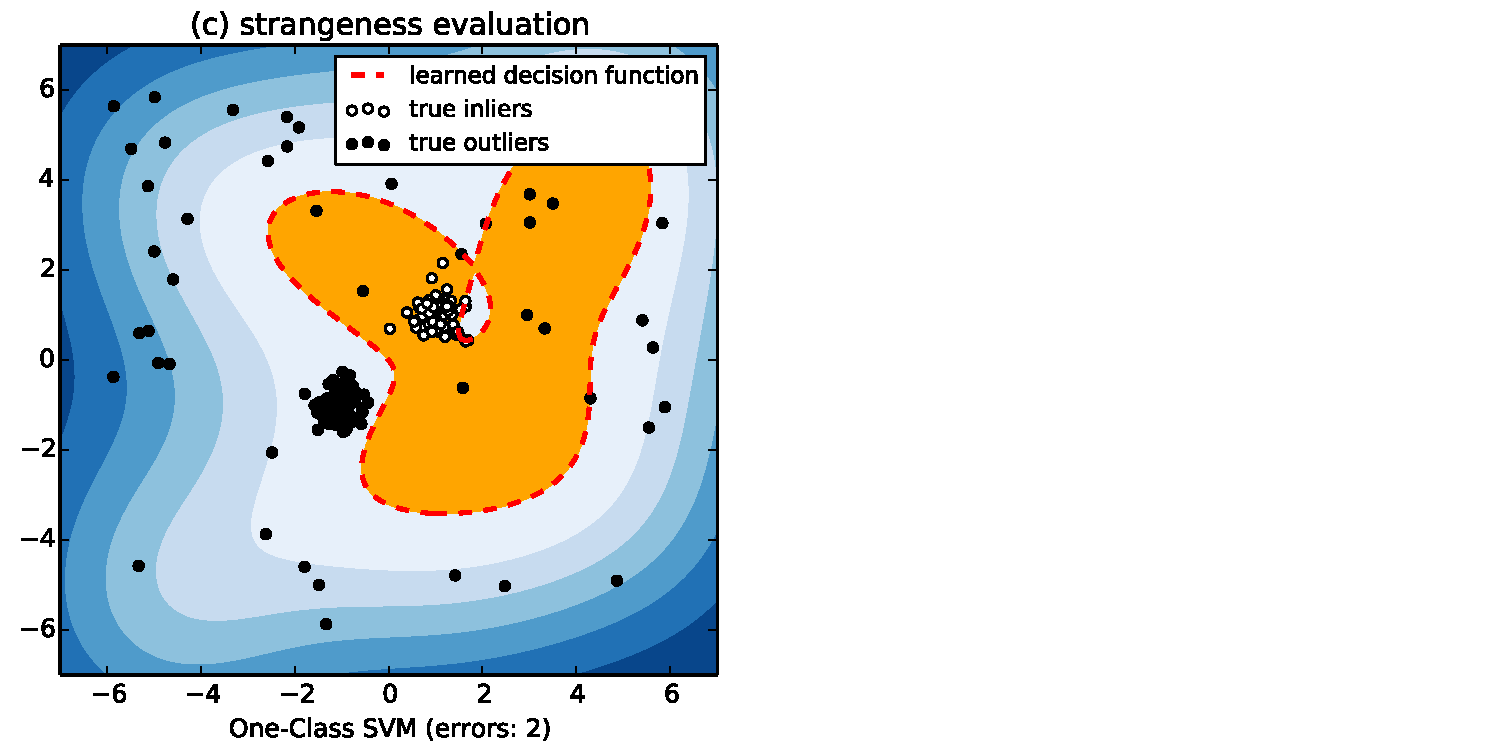
\includegraphics[width=6cm]{Figures/one_class/c}
    \centering
\endminipage\hfill
 
\caption[Plot of outlier detection in One-class classification]{Plot of outlier detection in One-class classification. (a) represents the initial dataset, (b) we have added new events that formed cluster, the plot represents the insterestingness evaluation, computing a model that takes into account all instances. The new event is inside the threshold, it is interesting (c) resprsents the strangeness evaluation test, the model is trained only with the normal instances from (a), the new event cluster is outside the thresold formed by the normal instances, it is considered strange. Example adapted from Scikit-Learn webpage \cite{scikit-learn}. \label{fig:plot_out}}
\end{figure}

This means that both steps, quantifying the strangeness and the interest of a stimuli can be solved with similar novelty detection processes and algorithms, only using different bases of knowledge.

\subsection{Model of normality}

The base of knowledge dataset will consist of all the poses ever presented to the system. The model of normality will be computed from this dataset.

\medskip

\centerline{ $ M(all.instances)$ formed by $ all.instances = [i_1, i_2, i_3,..., i_m]  $  }

The dataset will be expanded every time a new pose is presented to the system.

\subsection{Obtaining the noise score}

To differentiate it from the novelty score, we will name the score obtained to classify the entries as 'interesting' the $noise$ $ score$. If the entry is interesting, then it will have a low noise score.

We can obtain a fitting score, according to the algorithm, for each of the instances from the model $ M(all.instances) $ :
\medskip

\centerline{$ scores = [z(i_1), z(i_2), z(i_3),..., z(i_m)] $}

This set of scores represents a distribution of the scores of all entries. This distribution can be normalized, again as shown in Figure \ref{fig:normal_d}, obtaining a mean $\mu$ and a standard deviation $\sigma$.

Following the same procedure as in the previous section, we can obtain a standardized noise score.
 
\begin{equation}
noise.score(o_1) = abs( \dfrac{z(o1) - \mu}{ \sigma})
\end{equation}
 
\subsection{Obtaining the noise threshold} 

\label{thres2}

Following the same procedure as in subsection \ref{3.1.3}, we can obtain the formula:

\begin{equation}
noise.score(o_1) = abs( \dfrac{z(o_1) - \mu}{ K \times \sigma})
\end{equation}

This K factor, representing the units of standar deviation , $\sigma$, considered.

As seen in subsection \ref{3.1.3} we can declare 1 as the threshold for the noise score.

\section{Enabling the system to control the curiosity level} \label{3.3}

In the formula used to calculate the strangeness and noise score in Equation 3.6 and 3.10:

\begin{equation}
strangeness.score(o_1) = abs( \dfrac{z(o_1) - \mu}{ K \times \sigma})
\end{equation}

The value of K represents where we place the extreme values in the scores of the normal set, the threshold. If we develp the expression, it also represents the units of sigma considered, simplifiyng the threshold to a values of 1. By increasing the value of K, we increase the range fo the extreme values as shown in Figure \ref{fig:normal_d}. Table \ref{tab:sigma} summarizes the percentage of normal scores considered, and where we consider the extreme value, depending on the value of K.

\begin{table}[h]
    \begin{tabular}{ c  c }
    K value & Percentage \\ \hline
    1 & 68 $ \% $ \\ 
    1.98 & 95 $ \% $ \\ 
    2.58 & 99 $ \% $ \\ 
    \end{tabular}
    \centering
    \caption[Change in the percentage of normal scores considered depending on the value of K multiplying $\sigma$]{Change in the percentage of normal scores considered depending on the value of K multiplying $\sigma$, as presented in Figure \ref{fig:normal_d} \label{tab:sigma}.}
\end{table}


This K factor, as we have seen, can be applied to both strangeness and interestingness evaluation. We have named it the $curiosity$ $ factor$, and will serve as a way to modify the novelty score threshold. This is key to the sensityvity of the system. We can increase the sensitivity by decreasing the curiosity factor, because, to be normal, the new score will need to be very close to the mean with respect to all other instances in the base of knowledge.

As the value of the $cusiosity$ $factor$ depends on the sensitivity degree we want to achieve, and also on the nature of the data in te application, it needs to be commputed empirically.

\section{Enabling the system to learn from novel stimuli}

\begin{figure}[h]
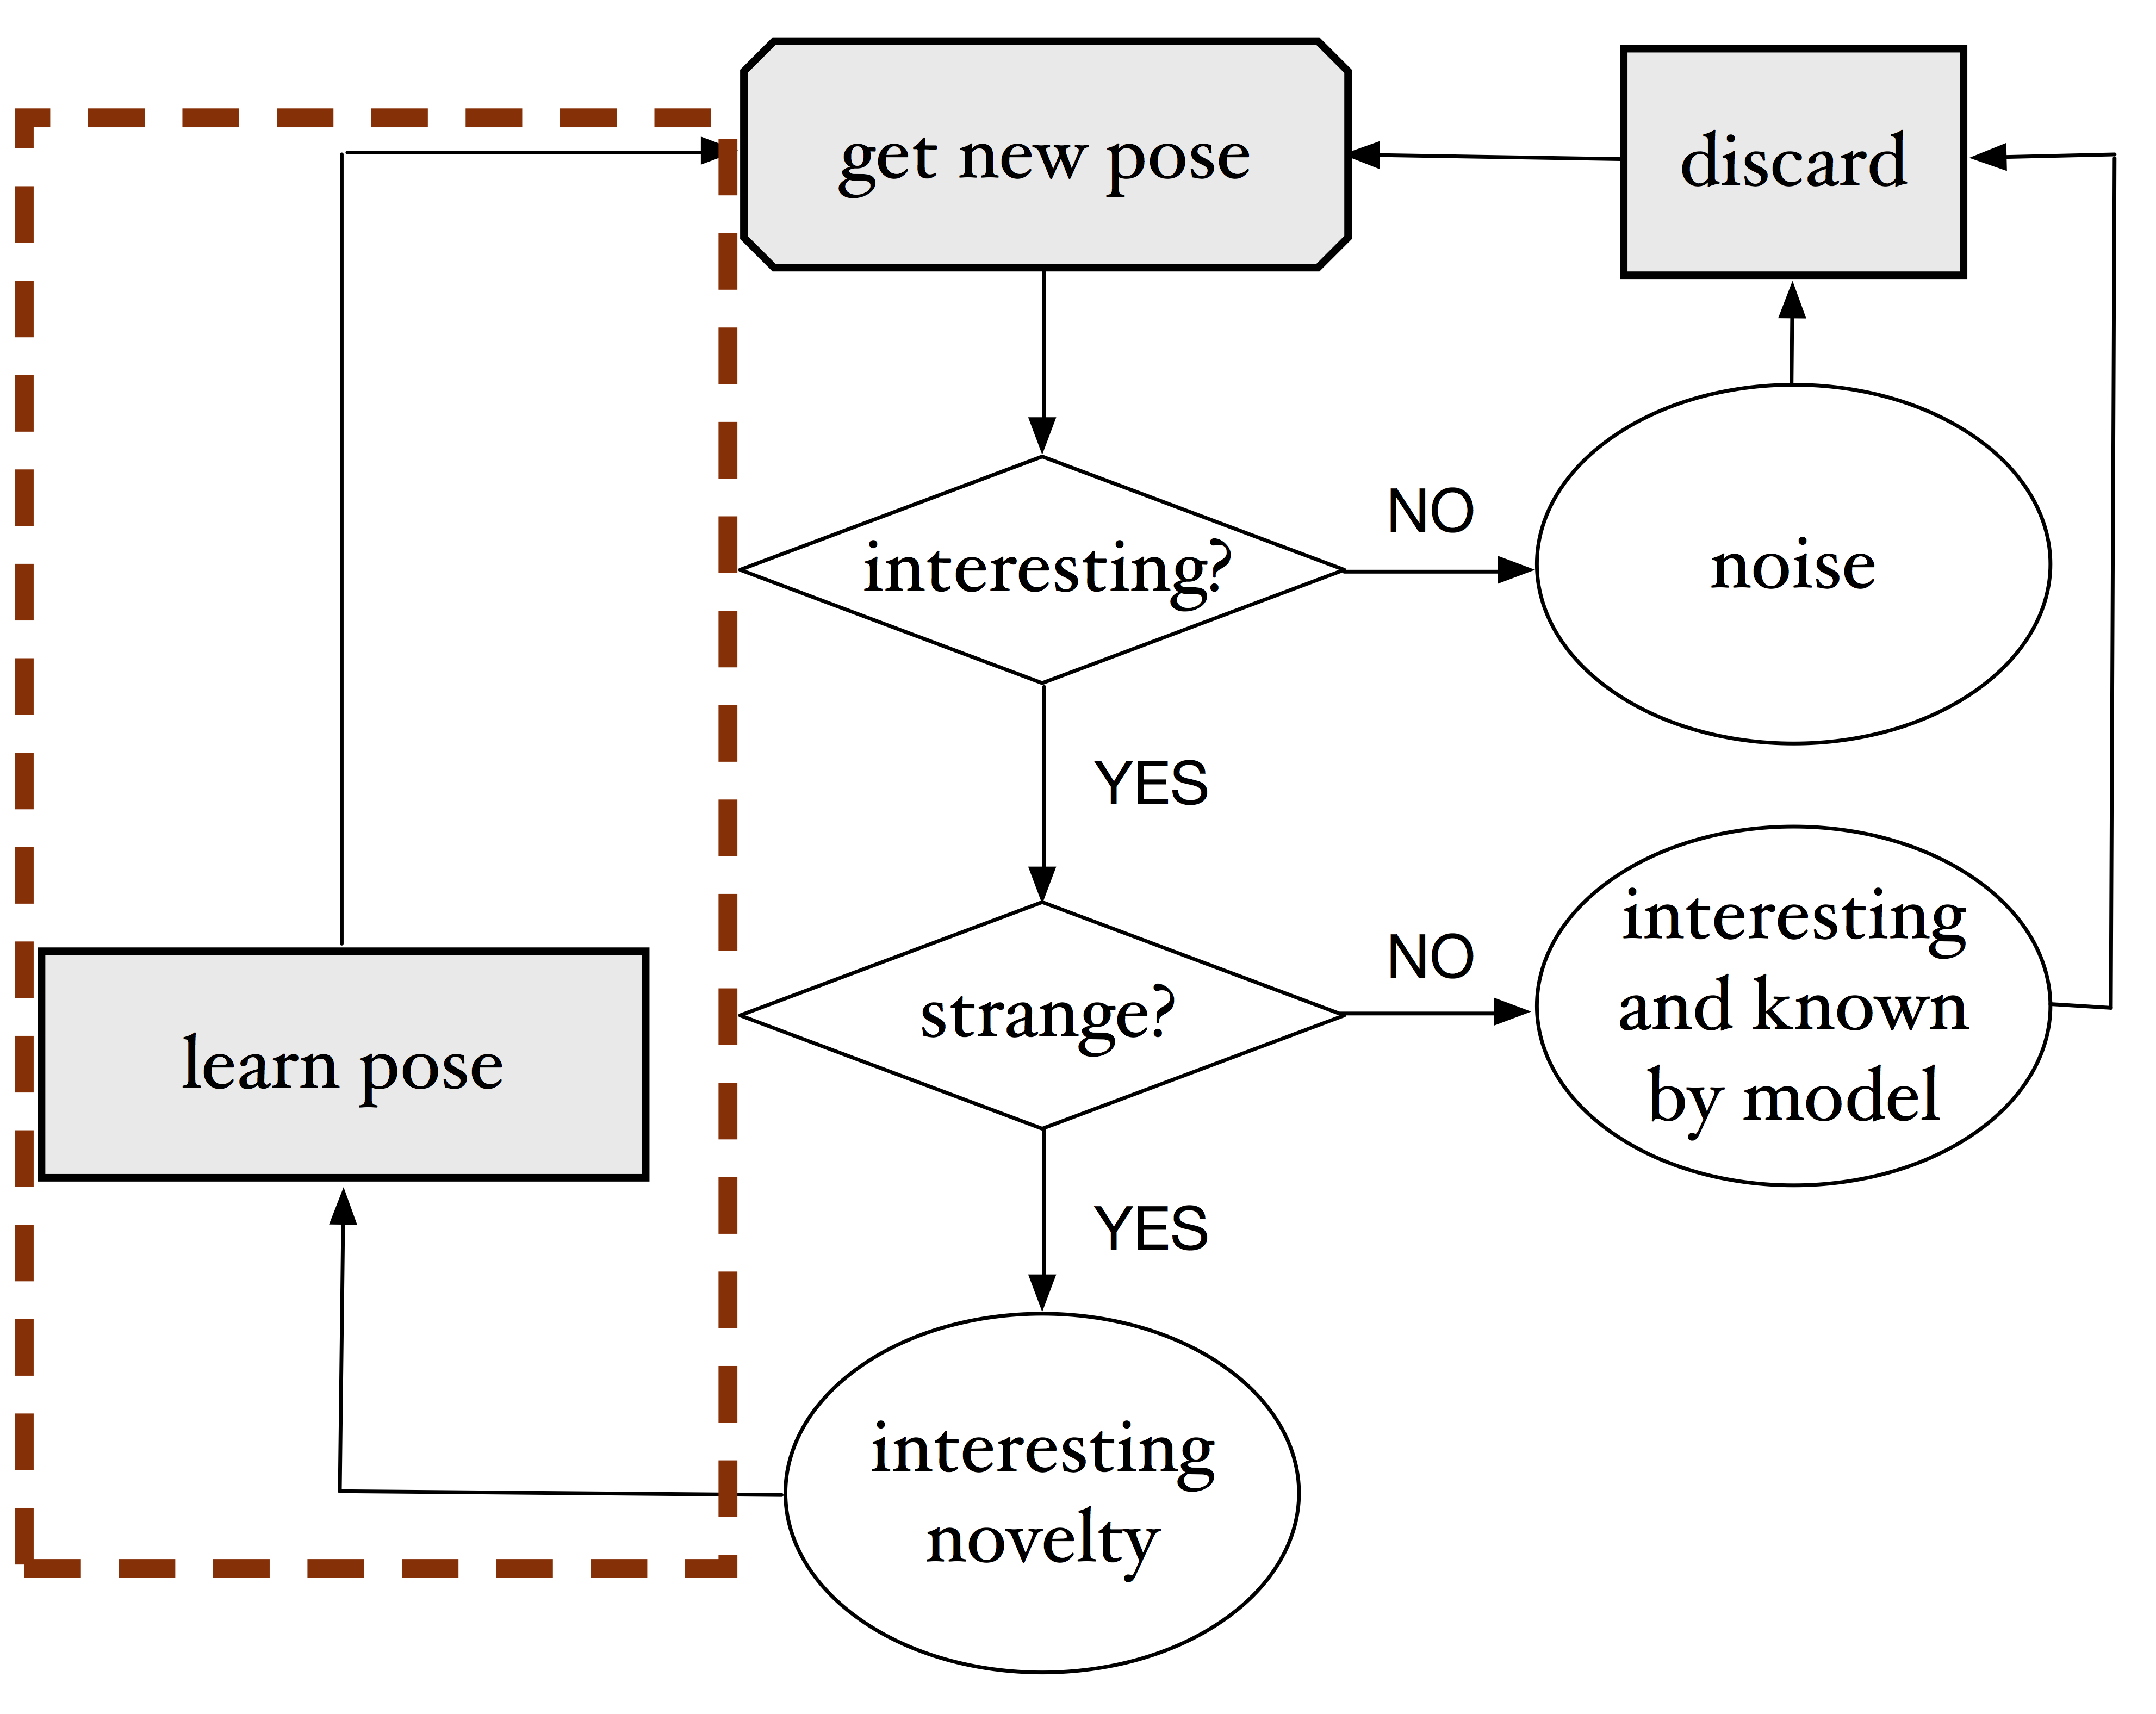
\includegraphics[width=9cm]{Figures/Esquema_learn}
\centering
\caption{Learning step located in the general scheme. \label{fig:scheme_learn}}
\end{figure}

The step of learning from novel stimuli is placed right after the data is classified as a \emph{novelty}, as seen in \ref{fig:scheme_learn}. The process consists of adding the novel data to the base of knowledge, the normal data set. After that, the Model of normality must be recalculated and expanded. A new score will be added to the set of normal scores and the mean $\mu$ and the standard deviation $\sigma$ will de recalculated as well.

A key concept in this step is avoiding misclassification. Building a model on misclassification can lead to future errors in the learning process. This can be avoided by asking the user when a novel entry is detected. By doing this, we can also ask for a label for the pose. The system will tell the user 'I don't know what you are doing. What are you doing?'. This confirmation will also be helpful to calculate the false alarm and the detection rate of the system. As mentioned before, the interaction with the user is out of the scope of this Thesis. However, the interface of the system has a 'Learn pose' button that allows the programmer to decide which poses to learn.

\section{Enabling the system to work autonomously and to be interactive}

The last step in building the system is that all this presented solutions have to be integrated in a system that works autonomously. Figure \ref{arch} displays the proposed software and hardware architecture for the system. It is important to remember that this process is a continuous closed loop, as shown in Figure \ref{fig:scheme}. In the architecture we only show the flow of data, so the closed loop is not explicitly drawn, since it means only waiting for a new input entry.

\begin{figure}[h]
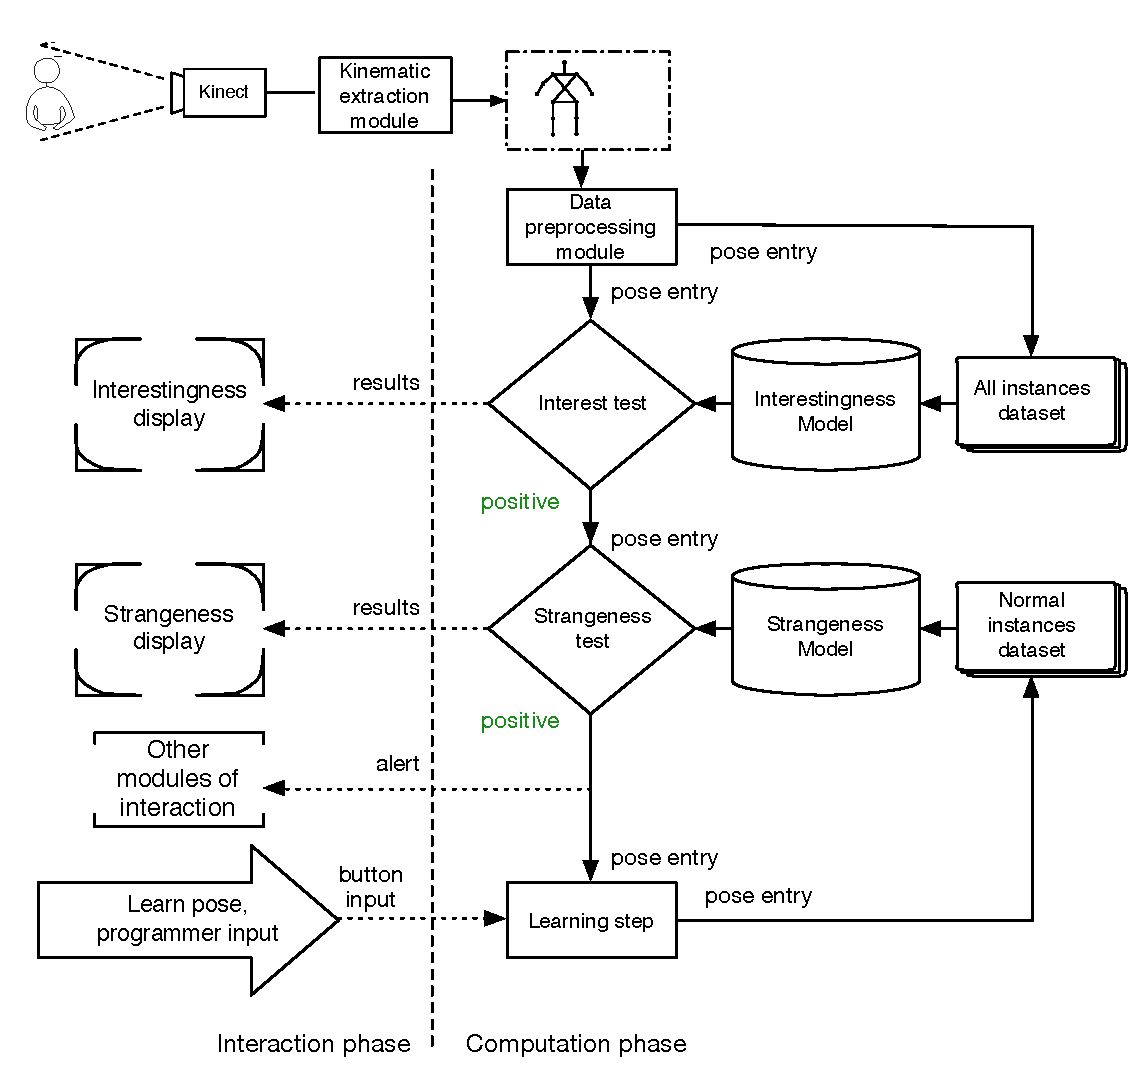
\includegraphics[width=14cm]{Figures/architecture}
\centering
\caption[System software and hardware proposed architecture]{System software and hardware proposed architecture\label{arch}. The skeleton-shape entry from the modules of the Kinect is preprocessed and saved in the \emph{all instances} dataset. It is then tested for interestingness and strangeness, and the results are displayed to the programmer. If the entry passes both tests, the system has found and novelty and alerts the programmer and other modules of interaction to ask the user. The programmer chooses to learn or not the novel pose by the button input 'Learn pose', that leads to saving that novel pose in the \emph{normal instances} dataset, learning it. When either of the satasets is updated, the corresponding model is updated as well.}
\end{figure}

The process starts with the Kinect recording the user, and retrieving a skeleton-shape entry using a Kinematic extraction module. This work was already done in the Department of Systems Engineering in a previous project \cite{Gonzalez-Pacheco2013}. This entry, $I$, will be then preprocessed, so it can be analyzed by our system and it is saved in the \emph{all instances} dataset. The nex step, is that $I$ is tested against the constructed interestingness model to analyze if it is interesting. The intestetingness score is displayed to the user via a simple interface. If $I$ passes the test and is interesting, it is tested against the normal model, to verify if it is strange. The outcome of this second test is displayed to the user too. If $I$ passes both tests, it means that the entry is a novelty. The following step is communicating an alert to other modules, if necessary. The programmer is responsible of deciding if the system must learn the pose, via a button in the interface. The pose is learned by storing it in the \emph{normal instances} dataset. The models are reconstructed when the corresponding datasets change, for future operation. 

In future iterations of the system, the learning step will not need to be supervised by the programmer. This supervision is only temporal, and serves to monitor the operation of the system in this first version built for the Thesis. Also, the integration with other modules os interaction is an area of future work.

\section{Description of the used novelty detection methods} \label{3.6}

Novelty detection techniques can be classified in the following categories, according to \cite{Pimentel2014}: 
(i) probabilistic, (ii) distance-based, (iii) reconstruction-based, (iv) domain- based, and (v) information-theoretic techniques. \cite{Pimentel2014}. Each category has a series of advantages and disadvantages, and different computational costs. Since, there is no single universal method for novelty detection \cite{Nehmzow2013}, the choice if the appropiate algorithm depends on the task. In the Experiments Chapter, four algorithms have been chosen to test their novelty detection performance for the pose recongnition problem adressed. This section describes the algorithms chose. 

\subsection{Probabilistic-based novelty detection methods}

These techniques use probabilistic methods that often involve a density estimation of the \emph{normal}  class. An entry in a low density area indicate that there is probability of it being a \emph{normal}  object \cite{Pimentel2014}.

The method used in this category is \textbf{Gaussian Mixture Model}, a GMM.
A GMM is a probabilistic model that assumes all the data points are generated from a mixture of a finite number of Gaussian distributions with unknown parameters \cite{scikit-learn}.

This Thesis used the implementation of GMM provided by Scikit-Learn Library \cite{scikit-learn}. It does not provide  directly a \emph{normal} or \emph{abnormal} method, but it does provide a built-in function called $score$. The score represents the log probability of a sample under the model. 

\subsection{Distance-based novelty detection methods}

This category includes the concepts of nearest-neighbour and clustering analysis that have also been used in classification problems. It assumes that \emph{normal}  data are tightly clustered, while novel data occur far from their nearest neighbours. \cite{Pimentel2014}

This thesis tested one method from this category, \textbf{K-Means}. The K-means algorithm clusters data by trying to separate samples in n groups of equal variance, minimizing a criterion known as the ‘inertia’ of the groups. \cite{scikit-learn} This algorithm requires the number of clusters to be specified, in this case, as we are interested in a one-class classification, the number of clusters will be 1. The K-means algorithm aims to choose centroids C that minimize the within cluster sum of squares objective function with a dataset X with n samples \cite{scikit-learn}.

The K-means method was also implemented in the the Scikit Learn Library \cite{scikit-learn}. It does not provide a \emph{normal} or \emph{abnormal} label either. The score function in this case represents the opposite of the value of X on the K-means objective \cite{scikit-learn}.

\subsection{Domain-based novelty detection methods}

Algorithms in this category use domain-based methods to characterize the data for the model of normality. These methods typically try to describe a domain containing \emph{normal}  data by defining a boundary around the \emph{normal} class such that it follows the distribution of the data \cite{Pimentel2014}.

Methods used from this category are specifically categorized as "oultier detection methods", and provide directly a label categorizing test data as \emph{normal} or \emph{abnormal}.

One of the algorithms chosen was \textbf{One Class SVM}, from the Scikit Learn Library\cite{scikit-learn}. The One-Class SVM has been introduced to decide whether a new observation belongs to the same distribution as exiting observations (it is an inlier), or should be considered as different (it is an outlier). It requires the choice of a kernel and a scalar parameter to define a frontier. The RBF kernel is usually chosen although there exist no exact formula or algorithm to set its bandwidth parameter. This is the default in the scikit-learn implementation. The $\nu$ parameter, also known as the margin of the One-Class SVM, corresponds to the probability of finding a new, but regular, observation outside the frontier \cite{scikit-learn}.

The other algorithm used is \textbf{Least Squares Anomaly Detection}. It is a flexible, fast, probabilistic method for calculating outlier scores on test data, given training examples of inliers. The model is controlled by two parameters: sigma (a kernel length scale, controlling how 'smooth' the result should be) and rho (a regularisation parameter, which controls the sensitivity to outliers) \cite{lsa}. It was implemented by John Quinn from Makerere University, Uganda.

\begin{flushright}

\end{flushright}